
\section{Introduction}

%%Video analytics is important, examples, organizations have hundreds of cameras
%%Video analytics is coming of age, powered mainly by deep convolutional neural networks (\nn), and automating large-scale analytics of video data that has so far relied on human inspection. 
Many enterprises and cities (e.g.,~\cite{videonews1,videonews2}) are deploying thousands of cameras and are starting to use video analytics based on deep convolutional neural networks (NN) for a variety of 24$\times$7 applications, such as traffic control, security monitoring, and factory floor monitoring. This trend is fueled by the recent advances in computer vision (e.g.,~\cite{he2016deep,he2017mask}) which have led to a continuous stream of increasingly more accurate models for object detection and classification. 


%%Pipelines, implementations & knobs, define configuration, resource-accuracy variation
A typical video analytics application consists of a {\em pipeline} of video processing modules. For example, the pipeline of a traffic application that counts vehicles consists of a decoder, followed by a component to re-size and sample frames, and an object detector. The pipeline has several ``knobs'' such as frame resolution, frame sampling rate, and detector model (e.g., Yolo, VGG or AlexNet). We refer to a particular combinations of knob values as a {\em configuration}. 

The choice of configuration impacts both the {\em resource consumption} and the {\em accuracy} of the video application. For example, using high frame resolutions (e.g., $1080$p) enables accurate detection of objects but also demands more GPU processing. The ``best'' configuration is the one with the lowest resource demand whose accuracy is over a desired threshold. Accuracy thresholds are set by the applications, \eg traffic light control can function with moderate accuracy of the analytics output while amber alert detection requires very high accuracy. Configurations (meeting the accuracy threshold) can often vary by {\em many orders of magnitude} in their resource demands~\cite{videostar,mcdnn}, and picking the cheapest among them can significantly impact cloud compute cost.
%%The best configuration is time-variant; give examples

The best configuration for a video analytics pipeline also {\em varies in time}, often at a timescale of minutes or even seconds. For the traffic pipeline described above, we may use a low frame-rate (\eg 5 frames/sec instead of 30 fps) when cars are moving slowly, say at a traffic stop, consuming $6\times$ fewer resources without impacting the accuracy of the vehicle count. In contrast, using a low frame-rate to count fast-moving cars will significantly hurt the accuracy. 

As such, we need to frequently change the configuration of the pipeline to minimize the resource usage while achieving the desired accuracy. While prior video analytics systems~\cite{videostar,noscope,zhang2015design,mcdnn} profile the processing pipeline to minimize cost, they only do so \emph{once}, at the beginning of the video. As a result, these systems fail to keep up with the intrinsic dynamics of the resource-accuracy tradeoff, and they end up either wasting resources (by picking an expensive configuration) or not meeting the accuracy target.

%%Given the large space of configurations, periodic exhaustive profiling is prohibitive. Negates the benefit.. (give example numbers)
One natural approach to address this challenge is to {\em periodically profile} the pipeline configurations to find an optimal resource-accuracy tradeoff. Unfortunately, this is prohibitively expensive because the number of possible configurations is exponential in the number of knobs and their values. Even a simple video pipeline with just a few knobs can have thousands of potential configurations. Further, the cost of executing some of the configurations can be orders of magnitude higher than the most efficient one we will pick. In fact, in our early experiments, the cost of periodic profiling often exceeded any resource savings gained by adapting the configurations. The main challenge, thus, is to significantly {\em reduce the resource cost of periodic configuration profiling}.
%the main issue is that the space of configurations is exponentially large.  and exhaustively profiling them is prohibitively expensive. 


%%Our problem statement is to adaptively pick configurations over time but be inexpensive in profiling, and pick the best configuration. 
%Our objective is to adaptively pick the best configuration over time for video analytics pipelines to produce outputs with the desired accuracy at the lowest resource cost. 


%%Characteristics of cameras: config characteristics tend to stay, cameras see similar scenes. We use both. 
Unfortunately, using traditional modeling techniques such as Bayesian optimization~\cite{cherrypick}, multi-armed bandits~\cite{amazon-bandit}, or optimal experiment design~\cite{ernest} to update pipeline configurations in the granularity of seconds is very expensive due to the number of experiments required by these techniques. In fact, these techniques typically assume a stationary environment where the optimization only occurs once upfront or rarely (once a day). Our setting, however, is {\em non-stationary}. 

To address this challenge, we take a more direct approach that leverages domain-specific insights on the {\em temporal and spatial} correlations of these configurations.

%%Temporal: In each profiling iteration, we make profiling cheaper using temporal correlation. Golden config. 
\noindent{\bf Temporal Correlation:} While the best configuration varies over time, certain characteristics tend to persist. For example, the top-$k$ best configurations (cheapest $k$ configurations with accuracy above the desired threshold) tend to be relatively stable over time, for a small value of $k$. Similarly, configurations that are {\em really bad}---very inaccurate and/or very expensive---remain so over long time periods. %Finally, for configurations whose values can be ordered (\eg frame rates), we can learn thresholds beyond which the accuracy tends to {\em plateau}. For instance, the accuracy of tracking people in a relatively quiet hallway tends to stay flat (and high) above 15 fps. 
Thus, over time, we can learn both the promising and unhelpful configurations, and thus significantly reduce the search space. 
%\ga{Is this what we want to say?}

%%Spatial: While the best config varies over time, they do stay the same across cameras. Motivation/reasons. Spatial correlation technique. 
\noindent{\bf Cross-camera Correlation:} Cameras deployed in geographical proximity (\eg in the same city or building) and for similar objectives (\eg traffic counting) often share properties (\eg the velocities and sizes of objects) that affects the optimal configuration. Instead of searching for optimal configurations per camera feed, we can {\em amortize the profiling cost across multiple cameras}. Once we identify a good set of configurations for a video feed, we can reuse this set on the feeds of similar cameras deployed in similar environments. This can dramatically reduce the cost of profiling, especially for organizations deploying large fleets of cameras.

%% independence observation.
\noindent{\bf Independence of Configurations:} A central question in any supervised learning problem is how to obtain high-quality labels. One possibility is to use humans to label the video feeds. Unfortunately, this approach is both slow and unscalable. Instead, we use an expensive {\em golden configuration} to provide the ``ground truth'' for accuracy, following prior work~\cite{noscope, videostar, focus}. An example of such a configuration for a traffic pipeline is a resolution of 1080p, at 30 fps, using a full-blown Yolo model. However, to minimize the cost of running the golden configuration, which uses the best (and most expensive) values for all knobs, we rely on an empirical observation that knobs are typically {\em independent}. That is, for a given configuration knob, the relationship between its resource and accuracy is largely independent of the values of the other configuration knobs. Thus, in our profiler, where we measure the value of a given knob (\eg frame rate) by simply holding the values of the other knobs fixed.

%%System: Chameleon, Evaluation highlights 
In this paper, we leverage these observations to develop {\name}, a video analytics systems that optimizes resource consumption and inference accuracy of video pipelines, by adapting their configurations in real-time. We evaluate {\name} using live video feeds of five real traffic cameras, and demonstrate that compared to a baseline that picks the optimal configuration offline,
\name can achieve 20-50\% higher accuracy with the same amount of resource, or achieve the same accuracy with only 30-50\% resource (or 2-3$\times$ speedup).
%%We have encapsulated these ides into {\name}, a video analytics controller, that optimizes 
%resource consumption and inference accuracy of video analytics pipelines by adapting their \nn configurations in real-time (Figure~\ref{fig:overall}). Using live video feed of \fillme real traffic cameras, we demonstrate that \jc{TODO}

%%Contributions 
Our key contributions are as follows:\vspace{-.1in}
\begin{itemize}
    \item We show that continuous adaptation of \nn configurations of video pipelines leads to better resource-accuracy tradeoffs than one-time tuning. (\S\ref{sec:potential}) \vspace{-.1in}
    \item We identify and quantify the impact of spatial and temporal correlations on resource-accuracy tradeoffs. (\S\ref{sec:insights}) \vspace{-.1in}
    \item We present a suite of techniques
    to dramatically reduce the periodic profiling cost. (\S\ref{sec:algorithm})\vspace{-.05in}
\end{itemize}



\comment{
\textcolor{red}{\bf OLD}

% video analytics is coming to age
Video analytics is coming to age.
Modern computer-vision techniques, in the form of deep convolutional 
neural networks (\nn), are set to transform our life by automating 
large-scale analytics of video data that so far has relied on 
human-based inspection.
Indeed, many organizations~\cite{??,??} have piloted \nn-based 
analytics on thousands of video feeds from traffic cameras, dash 
cams, and drones on a 24$\times$7 basis.
This trend is fueled by intensive on-going research~\cite{??,??}
from the vision community constantly improving the inference accuracy 
by ever more complex \nn solutions.

% finding good config is the key to optimizing cost-accuracy tradeoff
Unfortunately, applying \nn to video data at scale can be prohibitively
{\em expensive}.
For instance, one needs a \$9K GPU or \$800/month cloud VM to run
an \nn model~\cite{??} on just a single live video feed with relatively 
low quality, e.g., 720p and 30fps (frames per second). 
Worse still, recent vision techniques have largely improved inference
accuracy at the expense of increased processing time and resource 
consumption~\cite{??}.
Such cost is clearly untenable, and therefore, any practical system 
for video analytics must strike a balance between {\em resource 
consumption} and {\em accuracy}.


\begin{figure}[t!]
\centering
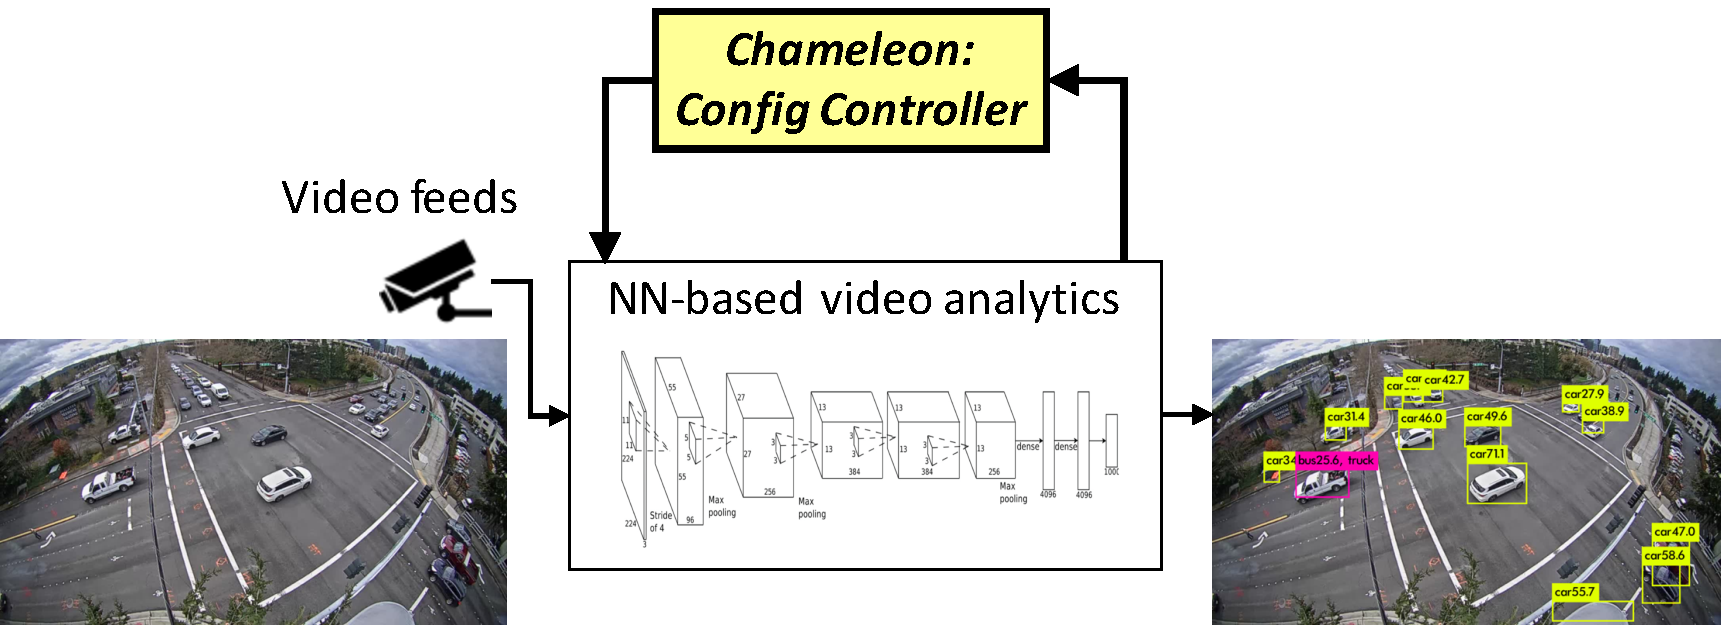
\includegraphics[width=0.5\textwidth]{PaperFigures/Overall.pdf}
\vspace{-0.2cm}
\tightcaption{Overview of \name, which features the configuration 
controller that continuously profiles and dynamically adapts the
\nn configurations.}
\label{fig:overall}
\end{figure}

We present {\em \name}, a video analytics controller, that optimizes 
resource consumption and inference accuracy of existing video 
analytics pipelines by adapting key \nn configurations in real-time.
(Figure~\ref{fig:overall}).
Prior work has observed that it is possible to reduce resource 
consumption with little cost in accuracy by using a cheaper \nn 
configuration (e.g., lower frame rate, resolution, and simplified
inference model)~\cite{videostar,noscope}.
However, to realize the full potential of tuning the \nn configurations,
the system must cope with the {\em intrinsic variability, both spatial
and temporal, in the resource-accuracy tradeoffs of \nn configurations}.
% The optimal configuration is sensitive to several characteristics
% that varies substantially over time and across video feeds.
For instance, any change in velocity of moving objects can alter
the optimal \nn configuration;
e.g., tracking cars within 5 meters at 30m/s (e.g., highway or 
off-peak hours) requires a frame rate of 6fps, but if cars are at 5m/s 
(e.g., crossroads or traffic jam), 1fps would suffice, 
an 84\% save in computing resources.
Many other factors, e.g., types and sizes of objects,
can similarly affect the resource-accuracy tradeoffs.
% In short, a flexible pipeline that self-adapts in realtime could 
% improve both resource consumption and inference accuracy.
Unfortunately, prior efforts only seek to find an optimal pipeline for
each query offline~\cite{videostar,noscope,vigil,mcdnn}, and thus fail
to exploit the intrinsic dynamics of the resource-accuracy tradeoff
which varies on much finer timescales (\eg seconds) than the video query
itself (\eg tracking objects for a week).

In contrast, \name continuously profiles the performance of different 
\nn configurations and adapts the \nn configuration in real-time
(\S\ref{sec:potential}). 
To analyze a video feed, \name starts with an offline-learned \nn 
configuration, periodically explores the configuration space
on a selected subset of video frames, and switches the configuration
when it identifies that a cheaper configuration can (or a more 
expensive one is needed to) achieve sufficient accuracy.

The key challenge in \name is that naively adapting the configurations 
requires searching an exponentially large configuration space 
periodically, which induces an overwhelming profiling cost that negates 
the gains of adaptation. This need to continuously re-optimize (\eg on 
the order of seconds) makes machine learning modeling approaches based on optimal experiment design~\cite{ernest}, Bayesian optimization~\cite{cherrypick}, or 
multi-armed bandits~\cite{amazon-bandit}, overly expensive, because these approaches 
assume a stationary environment where optimization only occurs once or daily. Our problem is {\em non-stationary}, and thus we take a more direct approach that leverages domain insights.

The insight behind \name to address the challenge is that while the 
underlying characteristics (e.g., the velocity and sizes of objects)
that affect the best configuration are dynamic, they show substantial
{\em temporal and spatial correlation} (\S\ref{sec:insights}).
For instance, traffic cameras often share properties (e.g.,
the distributions of velocities and sizes of objects) that affects
the choice of optimal \nn configurations, and such properties tend
to change slowly.

The temporal and spatial correlation enables \name to drastically 
reduce the profiling cost by amortizing it over time and across
multiple video feeds.
For instance, instead of searching for optimal configurations on a 
per camera basis, \name can amortize the re-profiling cost 
across cameras.
As long as we identify the best configuration one video feed, it 
can be used by other video feeds of similar cameras.
In scenarios such as traffic monitoring or surveillance video 
analytics, we indeed have concurrent video feeds from hundreds of 
cameras, many if not all of which are likely to share 
resource-accuracy tradeoffs of same configurations.

Amortizing the profiling cost, however, is easier said than done. 
In particular, one needs to check best \nn configurations learned
from certain video feed (or certain time window) is applicable to
to another video feed (or time window).
This turns out very onerous, because the accuracy (feedback) of 
applying an \nn configuration to a video feed is not instantly 
revealed; instead, it requires manually labeling or running a more
expensive configuration on the same video to get the ground truth.
Fortunately, for each configuration knob, the relationship between
its value and inference accuracy is largely independent to the setting on 
other configuration knobs (\S\ref{sec:algorithm}). This allows us to use 
a greedy hill climbing approach, where the value of each knob (\eg frame rate) is
tested and configured while holding the values of all other knobs fixed to some cheap value (\eg a cheap \nn model).

%In other words, to test a configuration on a video feed, we can
%test the value of each knob (e.g., frame rate) individually while
%fixing others to a cheap value (e.g., a cheap model). 

% how to {\em transfer} the best \nn configurations learned from one 
% video feed in one time window to a similar video feed or another 
% time window.
% \jc{i have two solutions for this part, but haven't decided which
% one works better. will add it later.}

Using live video feed of \fillme real traffic cameras, we demonstrate
that \jc{TODO}

Our key contributions are following:
\begin{itemize}
    \item We demonstrate that adapting \nn configurations in an online 
    fashion can achieve better resource-accuracy tradeoffs than 
    tuning configurations offline, though at a great cost of continuous 
    re-profiling (\S\ref{sec:potential}).
    \item We observe the spatial and temporal correlation of performance 
    tradeoffs (\S\ref{sec:insights}), and present a suite of techniques 
    (\S\ref{sec:algorithm}) to dramatically reduce the re-profiling cost.
\end{itemize}
}